
\documentclass{article}
\usepackage[spanish]{babel} %Definir idioma español
\usepackage[utf8]{inputenc} %Codificacion utf-8
\usepackage{amssymb, amsmath, amsbsy, wasysym}
\usepackage{multirow} % para tablas
\usepackage{graphicx}
\usepackage[ruled, vlined, spanish, linesnumbered]{algorithm2e} %Para escribir algoritmos
\title{Tarea 1\\Inteligencia artificial}
\author{Emmanuel Peto Gutiérrez}
\begin{document}
\maketitle

\section*{Reporte de algoritmos de búsqueda}

\subsection*{Instrucciones de uso}

El programa utiliza el lenguaje Java y como complemento se utiliza la biblioteca \textit{GraphStream} para visualizar gráficas. Para compilarlo es necesario tener instalado el \textit{Java Development Kit}, que incluye los comandos \texttt{javac} y \texttt{java}.

Como se tiene un archivo \textit{Makefile} se deben ejecutar los siguientes comandos:
\begin{itemize}
\item Para compilar: \texttt{make compile}
\item Para ejecutar: \texttt{make run}
\end{itemize}

Una vez que se ejecute se le pedirá al usuario que ingrese los datos necesarios para ejecutar algún algoritmo. Los datos que se le pedirán serán los siguientes:
\begin{itemize}
\item[1.] El nombre del archivo que contiene la gráfica. En este caso se llama \texttt{Rumania}.
\item[2.] El nombre del vértice de origen. Para el caso de Rumania es el nombre de alguna ciudad y es importante que la primera letra esté en mayúscula y el resto en minúsculas.
\item[3.] El nombre del vértice meta. Si se elige búsqueda voraz o $A^{\star}$ por defecto el destino será Bucharest.
\item[4.] Un número del 1 al 6 para elegir un algoritmo (en la consola se muestra cuál algoritmo representa ese número).
\item[5.] Si se elige búsqueda voraz o $A^{\star}$ se le pide que ingrese el nombre del archivo que contiene las distancias desde una ciudad hacia Bucharest. En este caso el archivo se llama \texttt{distancias}.
\end{itemize}

Una vez que se han proporcionados los datos adecuados, se ejecuta algún algoritmo y se muestra en consola el costo total del camino. Además, se muestra una gráfica del mapa donde las aristas rojas representan el camino recorrido por el algoritmo para ir del origen a la meta. Para terminar el programa basta con cerrar la ventana de la gráfica. En las siguientes imágenes se muestra un ejemplo.

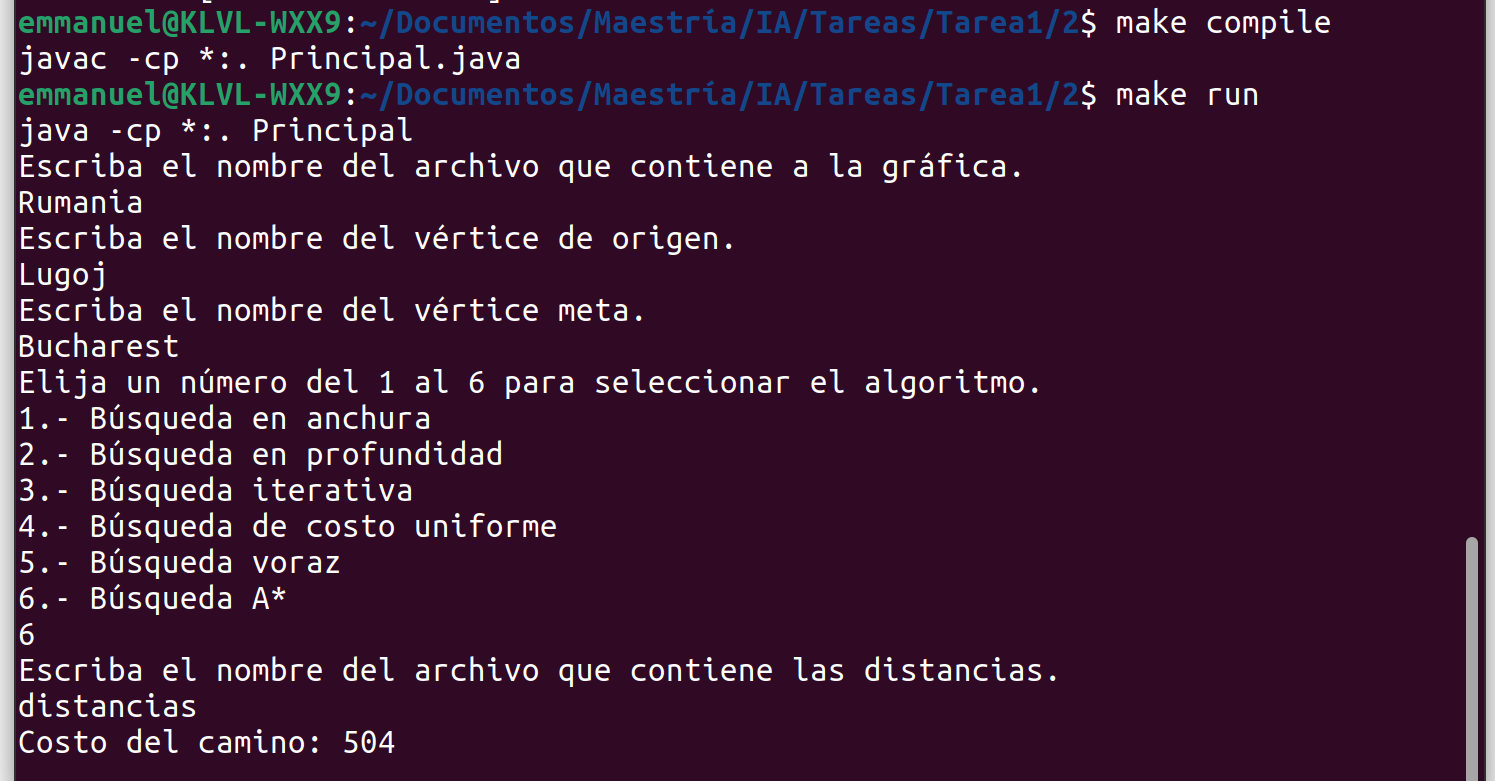
\includegraphics[width=0.8\linewidth]{consola.png}

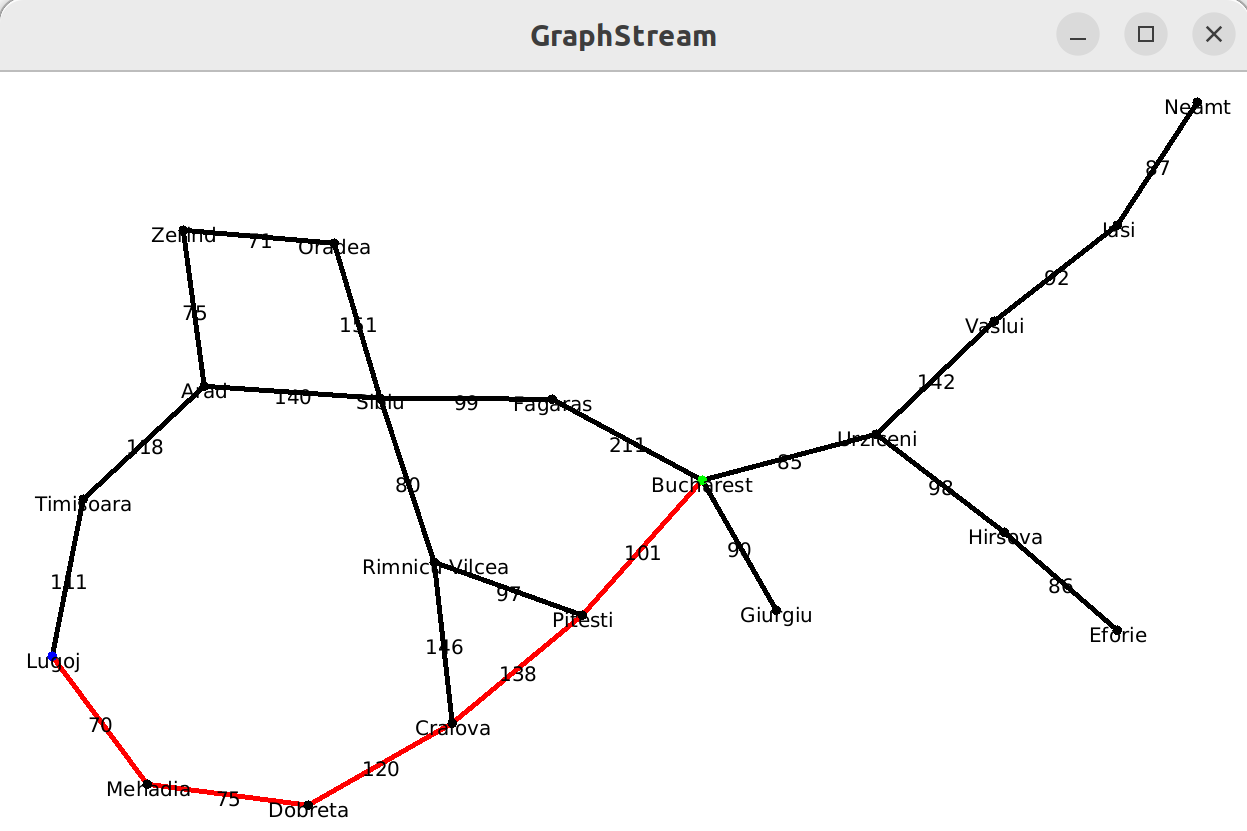
\includegraphics[width=0.8\linewidth]{grafica.png}

\section*{Resultados}

A continuación se muestran los resultados obtenidos con los diferentes algoritmos al hacer una búsqueda de Lugoj a Bucharest. Se muestra primero el camino y luego el costo del camino.

\begin{itemize}
\item[1)] \textbf{Búsqueda en anchura}: Lugoj $\rightarrow$ Timisoara $\rightarrow$ Arad $\rightarrow$ Sibiu $\rightarrow$ Fagaras $\rightarrow$ Bucharest. Costo: 679.

\item[2)] \textbf{Búsqueda en profundidad:} Lugoj $\rightarrow$ Timisoara $\rightarrow$ Arad $\rightarrow$ Sibiu $\rightarrow$ Vilcea $\rightarrow$ Pitesti $\rightarrow$ Bucharest. Costo: 647.

\item[3)] \textbf{Búsqueda iterativa:} El mismo que en \textbf{búsqueda en anchura}.

\item[4)] \textbf{Búsqueda de costo uniforme:} Lugoj $\rightarrow$ Mehadia $\rightarrow$ Dobreta $\rightarrow$ Craiova $\rightarrow$ Pitesti $\rightarrow$ Bucharest. Costo: 504.

\item[5)] \textbf{Búsqueda voraz:} El mismo que en \textbf{búsqueda de costo uniforme}.

\item[6)] \textbf{Búsqueda A$^{\star}$:} El mismo que en \textbf{búsqueda de costo uniforme}.

\end{itemize}

Se puede observar que en las búsquedas informadas se obtienen mejores resultados (por lo menos para el caso de Lugoj a Bucharest) que en el caso de las búsquedas no informadas.

\end{document}

